\documentclass[a4paper,12pt]{jsarticle}

\usepackage{amsmath,amssymb}
\usepackage{bm}
\usepackage[dvipdfmx]{graphicx}
\usepackage{verbatim}
\usepackage{wrapfig}
\usepackage{ascmac}
\usepackage{makeidx}
\usepackage{multirow}
\usepackage{here}
\usepackage{url}
\usepackage{comment}
\usepackage{arydshln}
\usepackage[top=35truemm,bottom=35truemm,left=25truemm,right=25truemm]{geometry}



\begin{document}

\setcounter{section}{3}
\section{各種調査、分析レポート等}

\subsection{投票率低下の原因調査及びVtuber利用の妥当性の検討}

図\ref{fig:voterate}に示すように現代の日本では選挙率の低下が問題となっており、特に若者の投票率が低い。図\ref{fig:vote}に示された投票に行かなかった理由から、投票率の低下の原因の大きな一つとして政治への関心が低いことが考えられる。

\begin{figure}[H]
	\begin{center}
		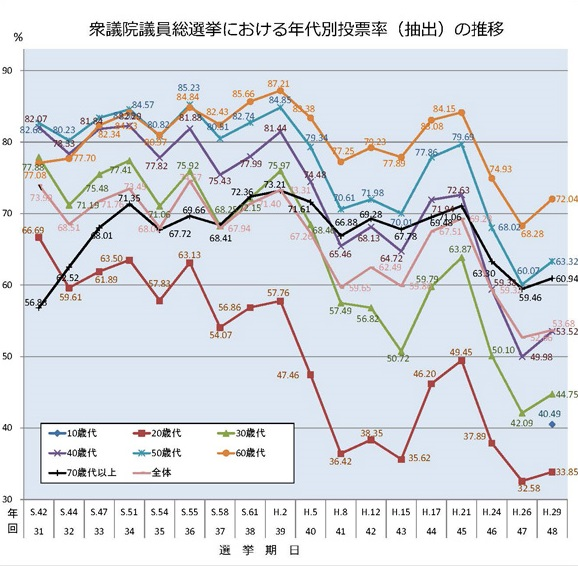
\includegraphics[width=12.0cm]{voterate.jpg}
		\caption{投票率の推移(出典 総務省\cite{vote1})}
		\label{fig:voterate}
	\end{center}
\end{figure}

\begin{figure}[H]
	\begin{center}
		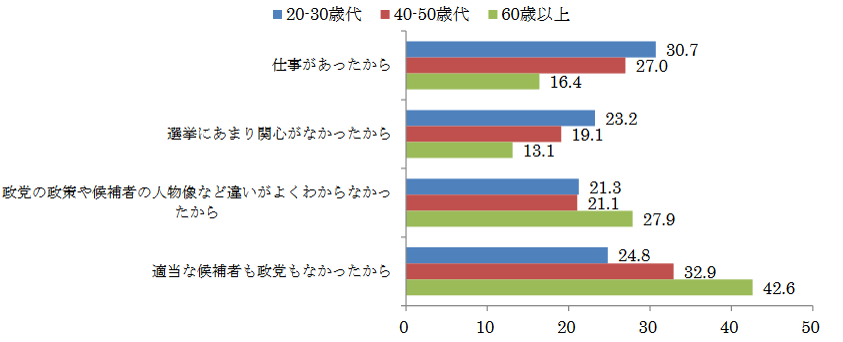
\includegraphics[width=12.0cm]{vote.png}
		\caption{投票に行かなかった理由(出典 財団法人明るい選挙推進協会\cite{vote2})}
		\label{fig:vote}
	\end{center}
\end{figure}

若者の投票率を上げるためには、若者に認知度があり興味のあるVtuberと選挙を紐づけることが効果的であると考えた。図\ref{fig:vtuber}に示すようにVtuberは若者の間で圧倒的な認知度を得ている。このことからVtuberを利用することで、若者の選挙への関心度の増加が見込める。

\begin{figure}[H]
	\begin{center}
		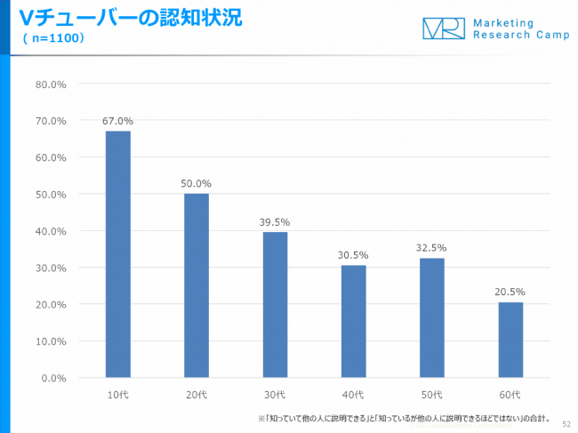
\includegraphics[width=12.0cm]{vtube.png}
		\caption{VTuberの認知状況(出典 MoguLive\cite{vtuber})}
		\label{fig:vtuber}
	\end{center}
\end{figure}

\subsection{政見放送に関する権利等の調査}

本システムでは政見放送の動画編集を行うため、政見放送の著作権及び公職選挙法を考慮する必要がある。

政見放送は著作権法第40条の定める「公開して行なわれた政治上の演説又は陳述」にあたり、「いずれの方法によるかを問わず、利用することができる」と解される。つまり、二次的利用(27条)も許され、同一性保持権の侵害にならない限り翻訳や要約も許される。また、他に複製物を譲渡すること(26条の2)ができる\cite{law}。選挙期間中に政見放送がYouTube等の動画共有サイトにアップロードされることが問題になることがあるが、これは著作権法上ではなく公職選挙法上の問題である。例えば、特定の候補者の政見放送のみをアップロードすることにより公平性が担保できなくなる、などの理由が挙げられる\cite{wiki}。

つまり、内容の同一性が確保された範囲での編集は可能であり、公平性が担保されていれば政見放送を利用することは可能であると考えられる。

\subsection{Google Cloud Speech-to-Text の使用料金}

本システムで使用したGoogle colud Speech-to-Textは60分まで無料で使用できるが、超過すると課金が必要でありその内訳を表\ref{tab:GCS2T}に示す\cite{GCS2T}。ここで示す標準モデルは音声を対象としたモデルであり、プレミアムモデルは動画、拡張音声電話にも対象を拡張したモデルである。本システムでは一番安価なコースを用いた。約五分の政見放送を対象とすると一回の使用料金は約8円となる。なお、開発の際は無料期間を利用したため使用料金は発生しなかった。

\begin{table}[H]
	\begin{center}
		\begin{tabular}{c|c|c}
			機能&標準モデル&プレミアムモデル\\ \hline
			音声認識(データロギングなし)&\$0.006/15[s]&\$0.009/15[s]\\
			音声認識(データロギングあり)&\$0.004/15[s]&\$0.006/15[s]
		\end{tabular}
		\caption{Google Cloud Speech-to-Text使用料金}
		\label{tab:GCS2T}
	\end{center}
\end{table}


\begin{thebibliography}{99}
	\bibitem{vote1} 総務省|参議院議員通常選挙における年代別投票率の推移 \\\url{https://www.soumu.go.jp/senkyo/senkyo_s/news/sonota/nendaibetu/}
	\bibitem{vote2} 財団法人明るい選挙推進協会|第46回衆議院議員総選挙全国意識調査p39\\\url{http://www.akaruisenkyo.or.jp/wp/wp-content/uploads/2013/06/070seihon1.pdf}
	\bibitem{vtuber} MoguLive|VTuberを10代の約7割が認知 ジャストシステムがリサーチを発表	\\\url{https://www.moguravr.com/just-systems-vtuber-research/}
	\bibitem{law} 栗田隆:著作権法注釈\\\url{http://civilpro.law.kansai-u.ac.jp/kurita/copyright/commentary/Act40.html}
	\bibitem{wiki} Wikipedia|政見放送 \\\url{https://ja.wikipedia.org/wiki/政見放送}
	\bibitem{GCS2T} Google Cloud|Cloud Speech-to-Text ドキュメント-料金 \\\url{https://cloud.google.com/speech-to-text/pricing?hl=ja}

\end{thebibliography}

\end{document}








